\documentclass{tufte-handout}

\title{Building support for improving transport: \\ Nine strategies \& a framework}

\author{James Reynolds, PTRG, Monash University}

%\date{28 March 2010} % without \date command, current date is supplied

%\geometry{showframe} % display margins for debugging page layout

\usepackage{graphicx} % allow embedded images
  \setkeys{Gin}{width=\linewidth,totalheight=\textheight,keepaspectratio}
  \graphicspath{{graphics/}} % set of paths to search for images
\usepackage{amsmath}  % extended mathematics
\usepackage{booktabs} % book-quality tables
\usepackage{units}    % non-stacked fractions and better unit spacing
\usepackage{multicol} % multiple column layout facilities
\usepackage{lipsum}   % filler text
\usepackage{fancyvrb} % extended verbatim environments
\usepackage{natbib}
  \fvset{fontsize=\normalsize}% default font size for fancy-verbatim environments

% Standardize command font styles and environments
\newcommand{\doccmd}[1]{\texttt{\textbackslash#1}}% command name -- adds backslash automatically
\newcommand{\docopt}[1]{\ensuremath{\langle}\textrm{\textit{#1}}\ensuremath{\rangle}}% optional command argument
\newcommand{\docarg}[1]{\textrm{\textit{#1}}}% (required) command argument
\newcommand{\docenv}[1]{\textsf{#1}}% environment name
\newcommand{\docpkg}[1]{\texttt{#1}}% package name
\newcommand{\doccls}[1]{\texttt{#1}}% document class name
\newcommand{\docclsopt}[1]{\texttt{#1}}% document class option name
\newenvironment{docspec}{\begin{quote}\noindent}{\end{quote}}% command specification environment

\begin{document}

\maketitle% this prints the handout title, author, and date


\begin{marginfigure}%
  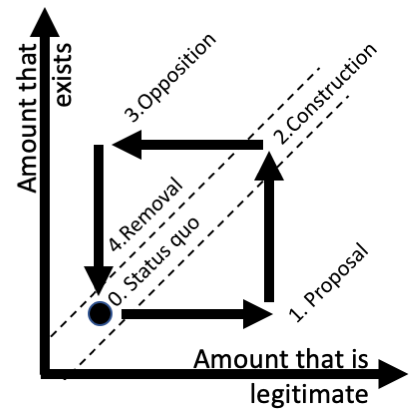
\includegraphics[width=\linewidth]{Framework_and_progression}
  \caption{Legitimacy framework and a simple progression}
  \label{fig:Legitimacy_framework}
\end{marginfigure}
  


\begin{abstract}
\noindent
Why is improving transport systems so hard? Roads and transit are typically under the control of political representatives, institutional bodies and (ultimately) the voting public, most of whom drive. Hence, the 'best' solutions from a transport engineering or planning perspective may not be feasible or even considered, otherwise excellent proposals may fail to be implemented, or beneficial improvements may face opposition upon construction and even later be removed for non-technical reasons. This handout outlines research findings\cite{Reynolds:2020aa}, including a new framework (Figure \ref{fig:Legitimacy_framework}) and nine pragmatic strategies
%\footnote{Building legitimacy before implementation through (A1) technical enquiry, (A2) transport planning or (A3) public processes; avoiding impacts through (B1) grade separation, (B2) new capacity, or (B3) subservience; and building legitimacy through implementation using (C1) bottom-up and incremental implementation, (C2) pop-ups, and/or (C3) trials.}%
that may help you implement projects and improve transport in the real-world of politics, NIMBYism and other non-technical challenges.
\end{abstract}

\smallcaps{Legitimacy} comes in many forms\footnote{Normative, sociological, through trust, through reasonableness, through unconditional duty, through public consent, or associated with conditional normative support.}. What is considered legitimate within the planning and engineering fields might be different to what is considered legitimate by the general public or within an institution such as a road authority. What is legitimate might also change over time, as shown in the simple progression shown in Figure \ref{fig:Legitimacy_framework}. Other progressions might lead to rejection of a proposal entirely, or a compromise in which what is ultimately built is provides less than what might be appropriate from a technical point of view\footnote{For example, passengers and traffic volumes may warrant a bus lane, but opposition might lead to construction of a High Occupancy Vehicle (HOV) instead} (see Figure \ref{fig:Failure_or_compromise}).


\begin{marginfigure}%
  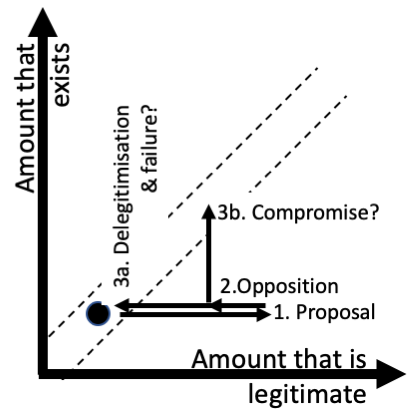
\includegraphics[width=\linewidth]{Failure_or_compromise}
  \caption{Failure or compromise}
  \label{fig:Failure_or_compromise}
\end{marginfigure}




\newthought{Nine pragmatic strategies} for legitimising implementation emerged from the case research described in this handout. The research looked at successful and not-as-successful implements of pedestrian malls, bicycle lanes and transit priority measures in Curitiba, Zürich, Boston, Toronto and Melbourne.  The first three strategies involve the \textbf{building of legitimacy before implementation}. This might take the form of (A1) \textbf{Technical Reporting}, with an objective of building support beyond just engineers and planners. Figure \ref{fig:Toronto_dashboard} provides an example from Toronto, where monthly dashboards during the King Street Transit Pilot contrasted the improvement in transit performance with impacts on pedestrians, cyclists, traffic and changes to economic activity. 

\begin{marginfigure}%
  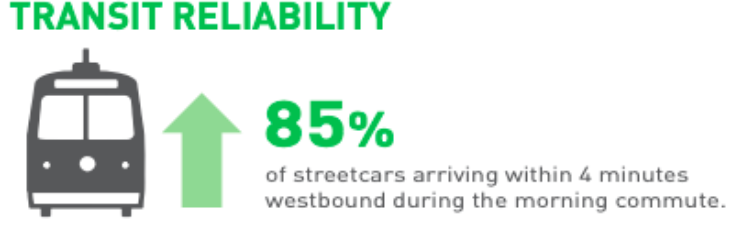
\includegraphics[width=\linewidth]{Toronto_dashboard_1}
   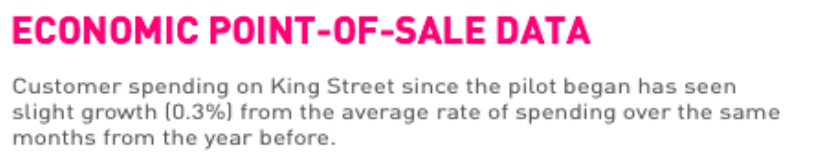
\includegraphics[width=\linewidth]{Toronto_dashboard_4}
  \caption{City of Toronto monthly dashboard during King Street Pilot (excerpt), see thesis p.274}
  \label{fig:Toronto_dashboard}
\end{marginfigure}

A (A2) \textbf{Transport Plan} can help build legitimacy, but research findings suggest that vision-based plans might be more likely to succeed. Curitiba's famous Bus Rapid Transit (BRT) network provides an example, having been supported by a vision for \footnote{The Plano Diretor} for transport and land-use to develop along linear 'Structural Axes'. In Zürich the Citizens' Transit Priority Initiative called for buses and trams to "travel along their lanes or tracks virtually as fast as is technically possible"\cite{Nash:2001ab}, which contrasts to the partially removed Stud Road bus lanes in Melbourne where the plan appears to have supported the specific objective of building the bus lanes. (A3) \textbf{Public Processes} might also be used, as in Zürich where the Citizens' Transit Priority Initiative narrow passed (51-49) in a public ballot. Ballots appear rare, but the research found cases were council meetings, environmental assessment hearings and other public processes (including even court hearings) appear to have legitimised implementation.  



\begin{marginfigure}%
  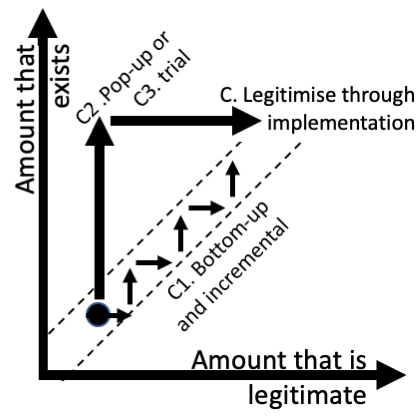
\includegraphics[width=\linewidth]{Figure4}
  \caption{Building legitimacy through implementation}
  \label{fig:FIgure4}
\end{marginfigure}







\newthought{But, why not simply avoid impacting} those who might oppose implementation?  This approach was successful for the Eglinton Crosstown LRT in Toronto, some of which is \textbf{B1. Grade-separated} so as not to impact traffic. In the context of Mayor Rob Ford's declaration that "the war on the car is over" putting the trams underground was the only way to get transit priority (even though very expensive). Similarly,  the Stud Road bus lanes were only removed where they had been converted from a traffic lane. Parts where they had been built as \textbf{B2. Additional Capacity} through road widening remain in place to this day.  \textbf{B3. Subservient priority} similarly seeks to limit opposition  by doing everything that can be done to help transit, but without impacting motorists, and is the genesis of Curibita's famous tubular bus stops and helps explains the retention of hook turns here in Clarendon Street. 

\newthought{Legitimacy though implementation} relates to the idea that “if they had a chance to actually see it, everyone would love it” (attributed to Curitiba's Mayor, Jamie Lerner\cite{McKibben:2007aa}). With \textbf{C1. bottom-up and incremental implementation} successive small changes are made, seeking to build on initial successes. The gradual addition of tram separation kerbing in the Melbourne CBD over the last (approximately) 20 years provides an example. \textbf{C2. Pop-ups} and \textbf{C3. Trials} provide other ways in which people can see what changes might look like in the real-world, without having to commit to permanence first.  For Jamie Lerner, it might help that he had the support of the military dictatorship ruling Brazil at the time his team converted central Curitiba into a pop-up pedestrian mall, but the guerrilla bike lanes of Seattle\cite{Fucoloro:2013aa} provide an example within democracies. At the least, as shown by Clarendon Street tram priority trial\cite{Silkstone:2005aa} and the King Street Transit Pilot in Toronto, temporary implementations can be used to find out which measures actually are legitimate enough to be kept.

Standards, technical analysis and other planning and engineering activity might help us determine what is technically appropriate. The research outcomes described here\footnote{And at length in the thesis!} might help you find out, and influence, what is legitimate in broader public policy-making arenas. 

\nobibliography{implementation_transit_priority_handout}
\bibliographystyle{plainnat}



\end{document}
